\section{DDoS Attacks and Defenses}
\label{ddos}

Denial of Service (DoS) attack: attempt to consume resources which are then not available to legitimate users. Possible target resources: network links, servers, processing, storage, etc. Distributed Denial of Service (DDoS) attack is a coordinated DoS with many attackers. DDoS attacks pose a significant threat and are often used to extort companies!

\subsection{Attack types}

\begin{minipage}{\linewidth}
    \centering      
    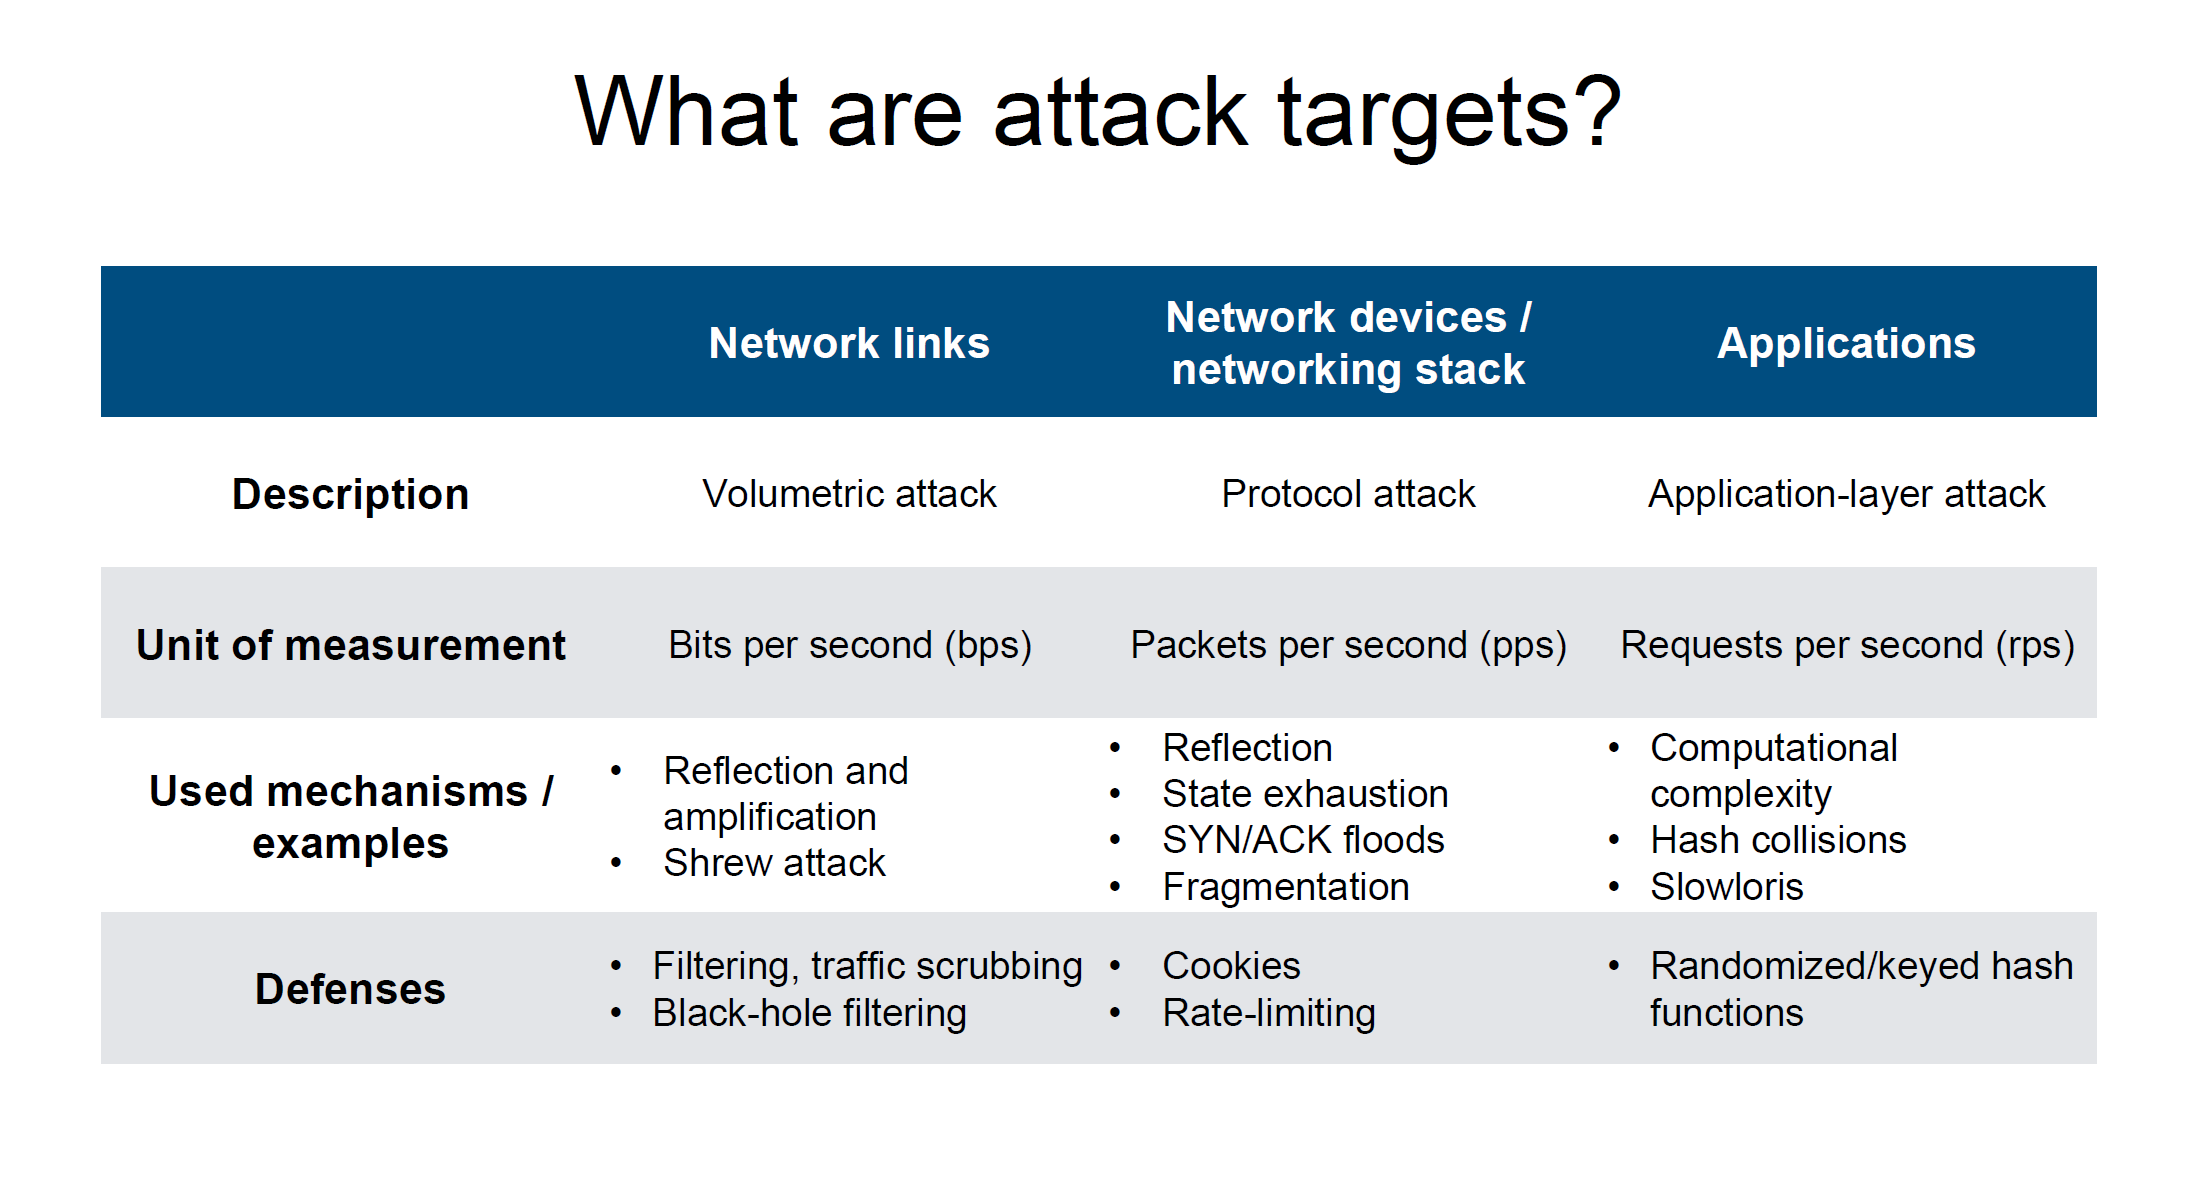
\includegraphics[width=\linewidth]{Figures/DDOS_attack_types.PNG} 
\end{minipage}

\subsection{(IoT) Botnets}
\paragraph{Botnet} 
\begin{itemize}
    \item A set of compromised machines connected to the Internet.
    \item Execute malicious code and can be controlled via command and control (C&C) systems.
    \item Often geographically distributed
\end{itemize}

\paragraph{IoT devices are perfect for constructing botnets}
\begin{itemize}
    \item Many devices with uniform configuration
    \item Often very poorly secured, hardcoded credentials.
    \item Often no security updates after few years.
    \item Often connected to internet without bandwidth limitations
\end{itemize}

\paragraph{Possible Mitigations:}
\begin{itemize}
    \item Patch: automatic security updates, provide patches for full life-time of devices.
    \item Credentials: No hardcoded credentials, force users to change default passwords.
    \item Monitoring: ISPs should actively monitor their network for suspicious traffic.
\end{itemize}

\subsection{Reflection and Amplification}

\paragraph{Address Spoofing:} Source address in IP header can be set by sender. In a connectionless protocol (UDP), server cannot confirm actual sender.

\paragraph{Defenses against address spoofing:}
\begin{itemize}
    \item Address filtering by ISPs: ensure hosts use their own addresses. Needs to be globally deployed. Poor incentives for ISP to deploy it (only other ISPs profit)
    \item Use connection-based protocols (TCP). Additional latency, potentially additional DoS attack vector (state exhaustion).
    \item Cryptographic source authentication: Additional DoS attack vector if built on expensive asymmetric crypto. Requires symmetric key distribution or PKIs
\end{itemize}

\paragraph{Reflection and Amplification:}
\begin{itemize}
    \item Requirements:
    \begin{itemize}
        \item Ability to spoof source address
        \item Publicly accessible servers
        \item Ideally response is (much) larger than request -> amplification
    \end{itemize}
    \item Typical reflectors:
    \begin{itemize}
        \item DNS (up to ~180)
        \item NTP (up to ~500) vulnerability was closed.
        \item Memcached (up to ~50000) UDP disabled by default in  version 1.5.6
    \end{itemize}
\end{itemize}

\begin{minipage}{\linewidth}
    \centering      
    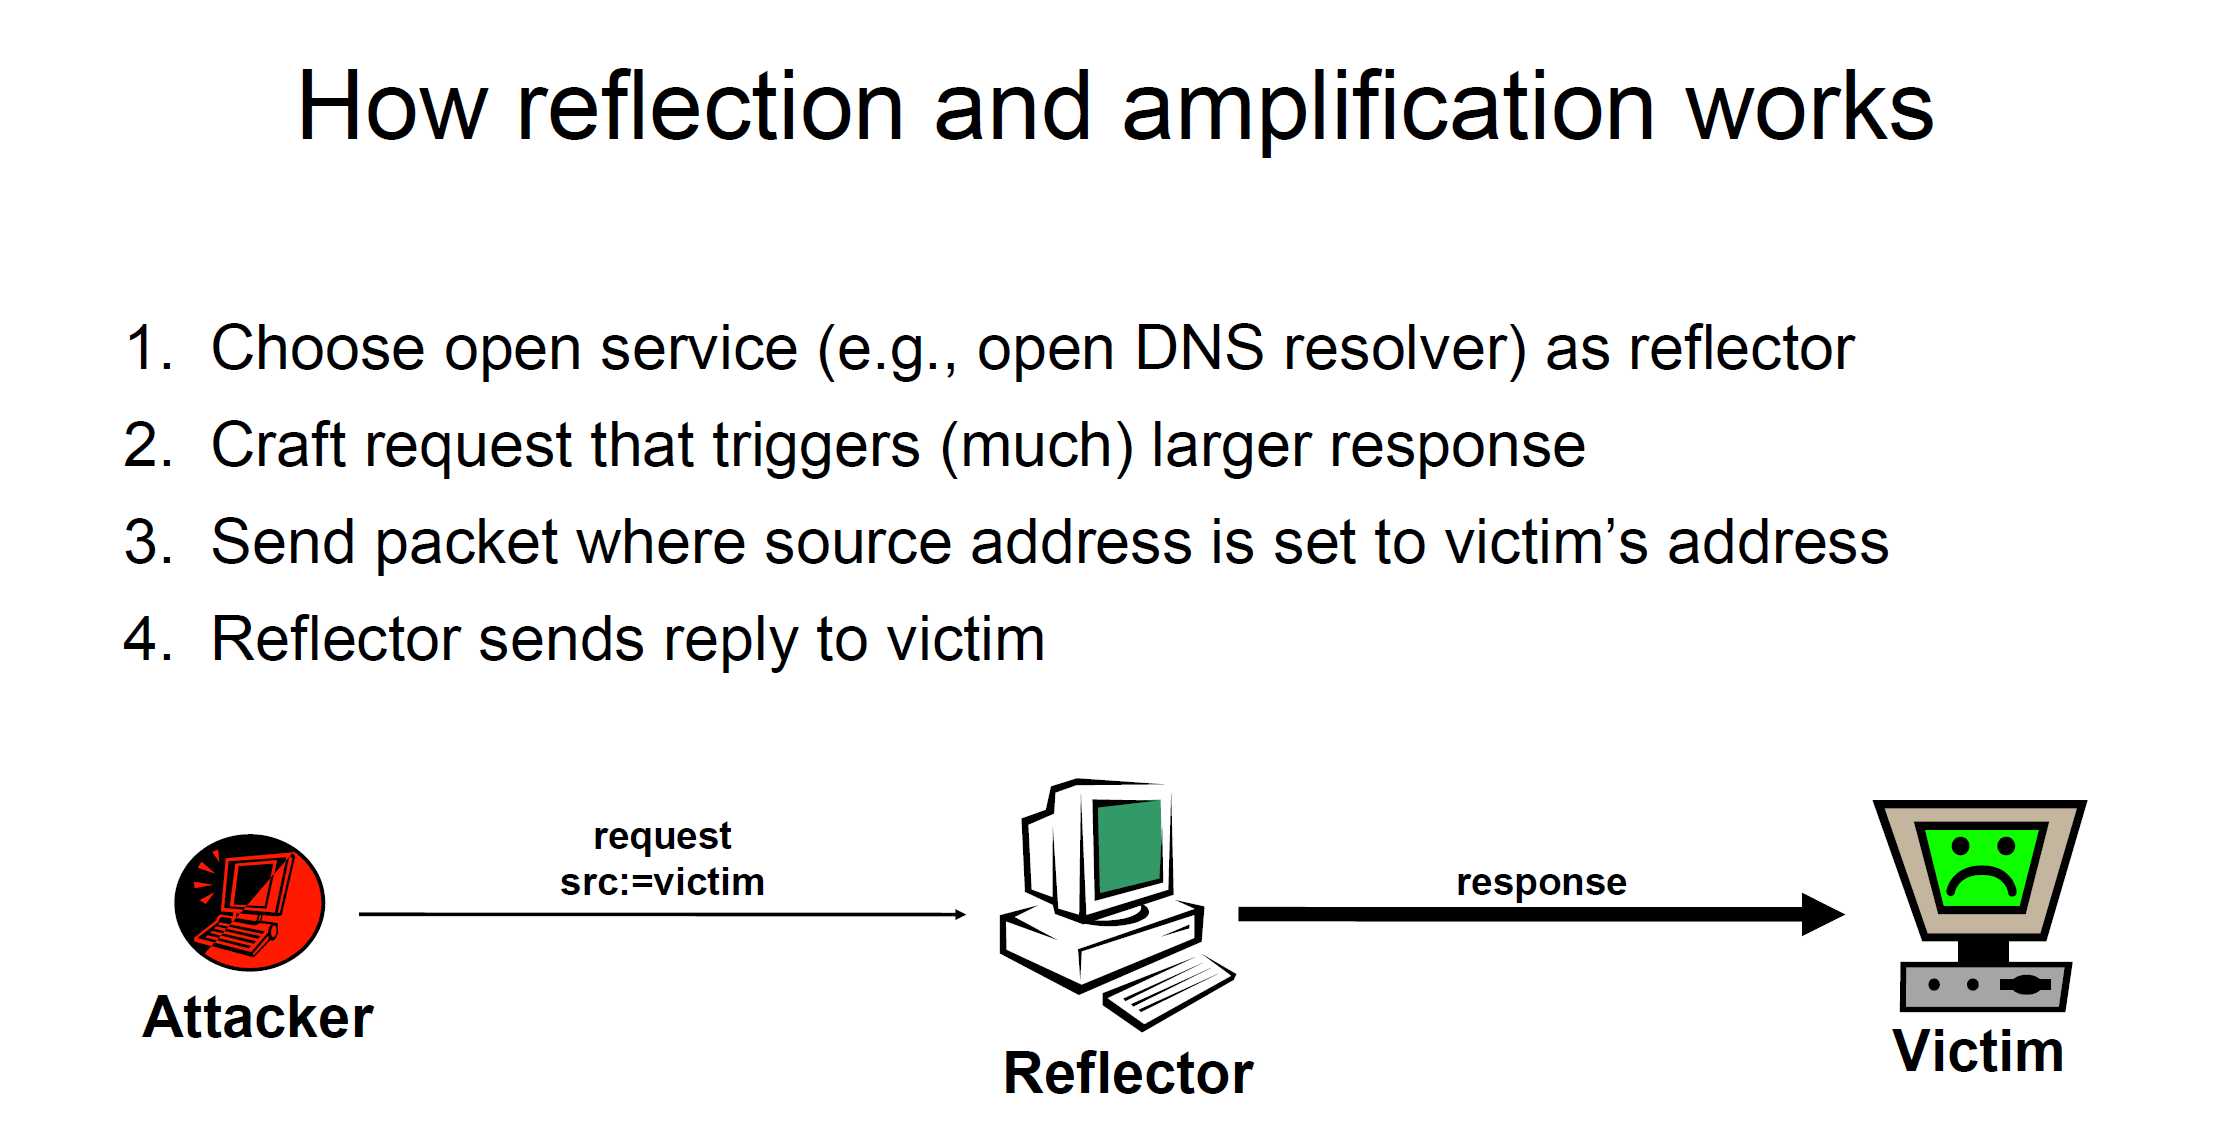
\includegraphics[width=\linewidth]{Figures/DDOS_reflection.PNG} 
\end{minipage}

\begin{minipage}{\linewidth}
    \centering      
    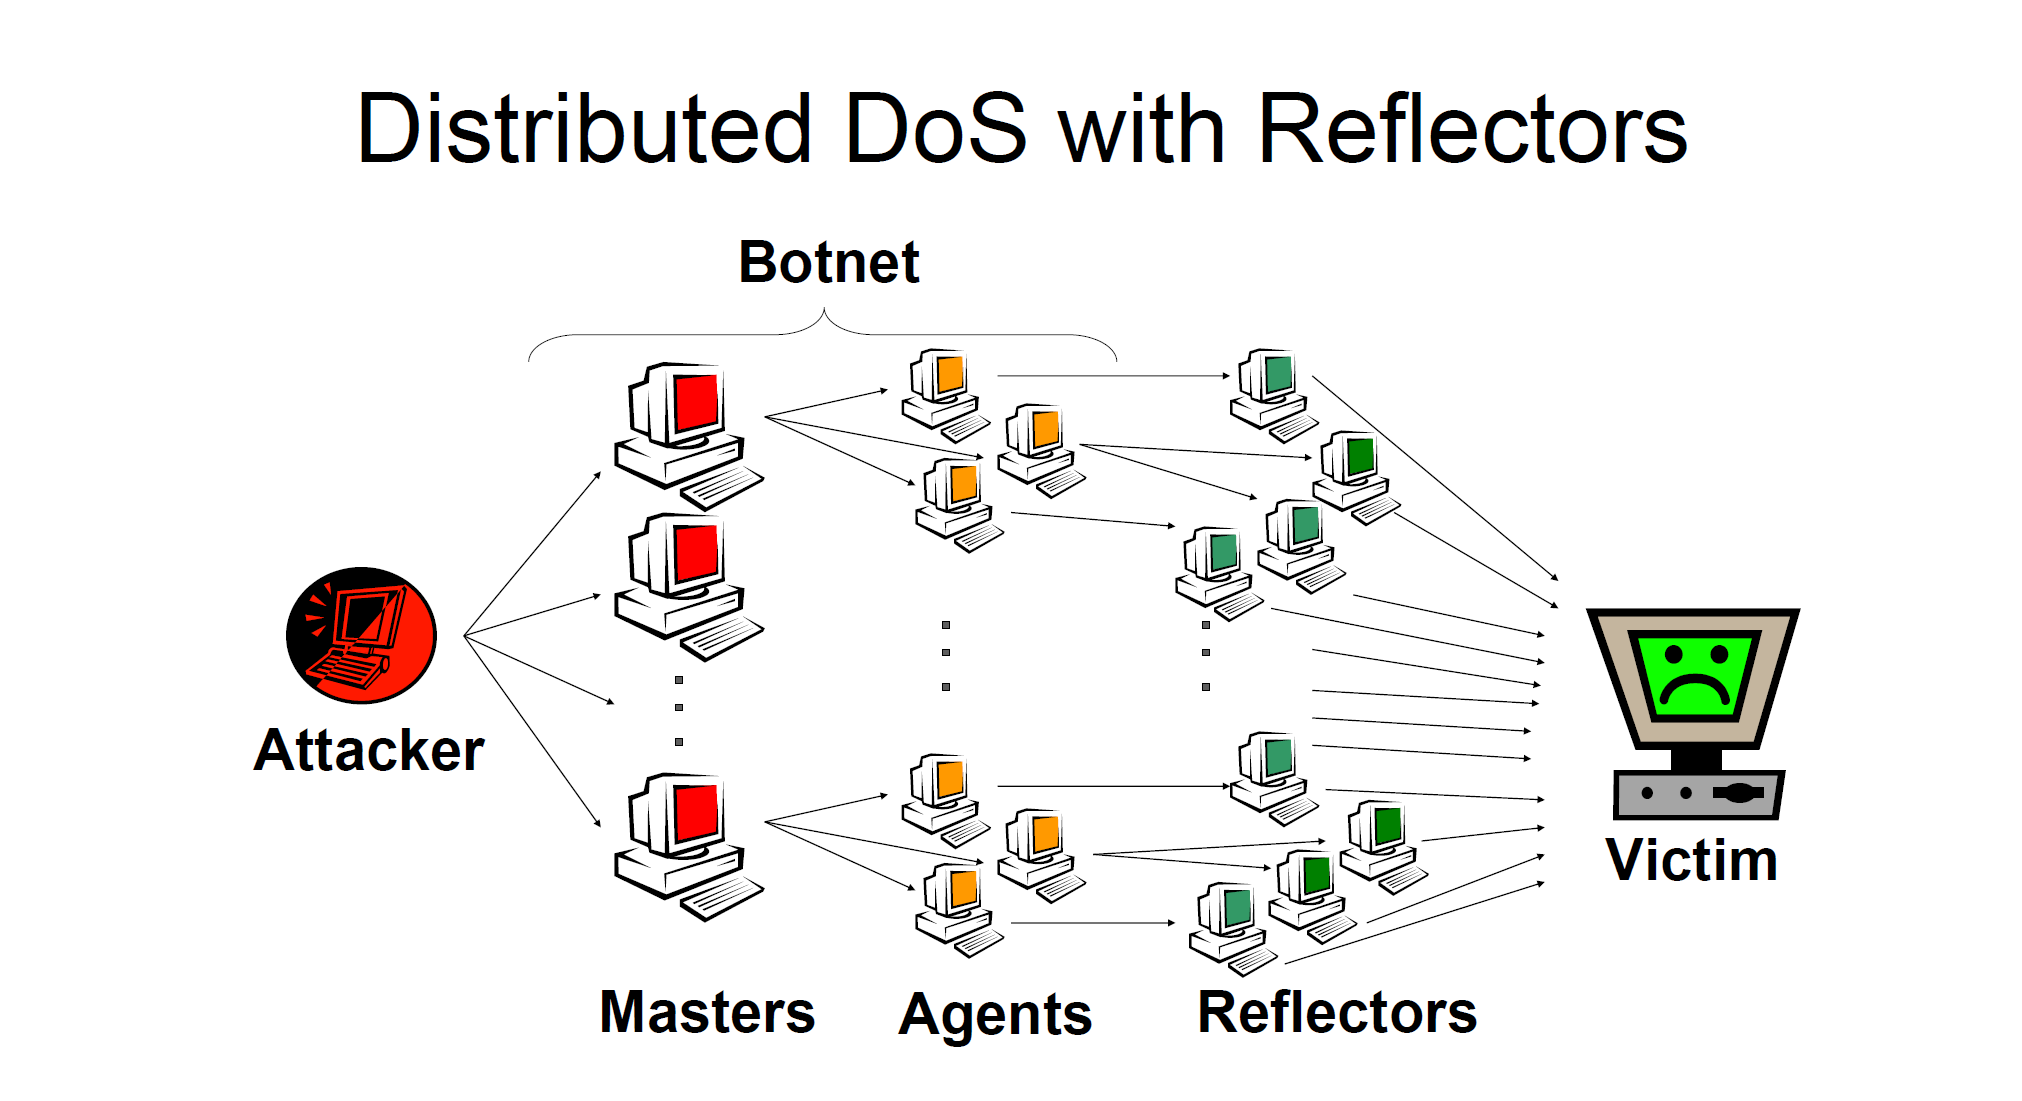
\includegraphics[width=\linewidth]{Figures/DDOS_distributed_reflection.PNG} 
\end{minipage}

\paragraph{Reflection Mitigations:}
\begin{itemize}
    \item Prevent address spoofing
    \item Perform access control (DNS servers deployed within an organization or ISP should only serve clients from this organization.
    \item Implement response rate limiting RRL (limit the nr of responses to a client)
    \item Ensure small amplifications factors (ideally < 1)
\end{itemize}


\subsection{Specific Attack Examples}

\subsubsection{Volumetric Attack: Shrew Attack}

Conventional bandwidth-based DoS requires sending high-rate attack traffic (like an elephant). Can we achieve the same effect by sending low-rate attack traffic (like a fierce shrew)? YES!\\

\paragraph{Shrew DoS Attack:} Exploits TCP congestion control feature. Researchers discovered that if you send traffic during very short but specific amounts of time, you can completely disrupt TCP. This is due to TCP congestion control resending packets at multiple whole seconds granularity (1s, 2s, 4s, 8s, ...). By only creating congestion during these time periods the attacker forces TCP flows to repeatedly enter a retransmission timeout state by sending high-rate but short-duration bursts! We deny the bandwidth of legitimate TCP flows as it makes TCP believe there is a long-term congestion.

\paragraph{Retransmission Timeout in TCP Congestion Control}
\begin{itemize}
    \item Exponential bakcoff timeout: If packet dropped retransmit in 1s, then 2s, then 4s...
\end{itemize}

\paragraph{Temporal lensing:} "multiple rounds simultaneous impact”. Use time as an additional amplification factor. Different paths have different transmission delays. An attacker can send packets at different times s.t. they \textit{all} arrive at the target \textit{at the same time}. So that a low-bandwidth source can also perform a shrew attack.

\subsubsection{Volumetric Attack: Coremelt and Crossfire}

Both of these attacks haven't been seen in the wild yet but are theoretically possible.

\paragraph{Coremelt attack}

\begin{itemize}
    \item Adversary controls many bots distributed across the Internet.
    \item Bots send traffic \textit{between each other}, thus all traffic they produce is legit traffic desired by the destination (destinations are bots). Traffic is not sent to a victim as in regular DDoS attacks. Thus, all defense methods discussed before do not work here.
    \item Adversary can exhaust bandwidth on victim link.
    \item As a result, the attack traffic exhausts bandwidth in per-flow fair sharing systems.
\end{itemize}

\paragraph{Crossfire attack}

\begin{itemize}
    \item Adversary controls distributed bot army
    \item Observation: due to rout optimization, few links are actually used to connect a target region to rest of internet. 
    \item Adversary can contact selected servers near/in target region to overload target links.
    \item Result: disconnect target region from remainder of Internet.
    \item Hard to stop since only connection establish packet (TCP SYN) are sent.
\end{itemize}

\subsubsection{Protocol Attack: DNS FLooding}

\paragraph{NXDOMAIN Attack}
\begin{itemize}
    \item Goal: overwhelm victim's authoritative name servers.
    \item Idea: query many non-existent subdomains of victim domain.
    \item Resolver queries all authoritative name serverss in turn
    \item Can use multiple DNS resolvers
    \item Can be sent from distributed botnet and via many different DNS resolvers.
    \item Result: name server can no longer reply to legitimate requests.
\end{itemize}

\paragraph{Why is this a problem?}
\begin{itemize}
    \item Most internet-based services rely on DNS to map domain names to IP addresses.
    \item If a domain name cannot be resolved, the service does not work.
    \item A DoS attack on the DNS system makes many additional systems unavailable.
\end{itemize}

\subsubsection{Protocol Attack: Session State Exhaustion}

\paragraph{Session State Exhaustion}
In a two way communication, each channel between peers needs a unique session number. This session number has to be known at the server to match requests to the right session/ channel. Keep in mind that servers have limited memory.\\
\noindent\textbf{Attack:} Exhaust the session table of the server.\\
\textbf{Result:} Server can no longer accept new connections, existing connections are dropped, maybe the server/service crashes.

\paragraph{SYN Flood Attack}
TCP uses a three-way handshake to establish a connection. The client initiates the handshake by sending a SYN packet. The server stores a new state for the received SYN packet.\\
\textbf{Attack:} The attacker can send lots of TCP SYN packets with spoofed srcIP. The server tries to keep state for every single packet. Eventually, the state table overflows and the server is unable to accept new legit connections. For each second where the packet is in buffer, its TTL is decreased by 1. It thus takes 255 seconds until the state is dropped.\\
\textbf{Mitigation:} SYN Cookies - no state table needed. Server doesn't create session state for TCP SYN packet. Instead, the server replies with SYN+ACK and a cookie (sequence number) $B=F(time,IP,port,...)$. On the next reply, the server then checks if the client sent $B+1$ along. Attacker can just send the cookie too...? No! Since the srcIP is typically spoofed, the attacker won't receive the cookie. The attacker could try to spoof the cookie (if she knows the function F...). The server should use cryptographic hashes or salted hashing such that the attacker can only guess $B$.

\paragraph{Generic Mitigations}
\begin{itemize}
    \item Attack: The attacker aims to exhaust session state of a protocol/application at server.
    \item Countermeasures:
    \begin{itemize}
        \item Encode state in a unique but determined way that allows the server to validate the state in the reply.
        \item No need to store session state at the server.
        \item Ensure the encoding cannot be tampered (use crypto-hashes, unique data known to server only)
        \item Server generates B = Hash(salt, A) where salt is known to server only and changes over time
        \item Server only needs to store a few salt values to validate replies.
    \end{itemize}
\end{itemize}

\subsubsection{IP spoofing defense}

\begin{itemize}
	\item Ingress Filtering: at network edge, outgoing packets with incorrect srcIPs are filtered (e.g. ETH filters packets whose srcIP is not within the ETH prefix). All ISPs should do this (in reality only 30\% do).
	\item iTrace: One in 20,000 packets “triggers” a router to send a special packet with route information sent to both src and dst. DDoS victim could reconstruct attack paths. But extra packets waste bandwidth.
	\item Packet Marking: Routers mark 16-bit IP ID field with information that enables reconstruction of IP address. This has no overhead but probabilistic marking often requires ca. 1000 packets.
\end{itemize}

\subsubsection{Application-Layer Attack: Algorithmic Complexity Attack}
Algorithms often have good average case running times but bad worst case running times (for certain inputs) (e.g. quicksort or hashtable lookup).\\
An attacker can exploit this by sending special inputs that trigger worst-case running times of algorithms.

\paragraph{Hash table lookup: Countermeasures}
\begin{itemize}
    \item Universal Hashing: Hash functions guarantee 0 or low collision for any input
    \item Hash randomization: Harder for attacker to find out the worst-case input. E.g. use a secret hash function for each hash table.
\end{itemize}

\subsubsection{Regular Expression Denial of Service (ReDoS)}
There are "malicious" inputs to certain regular expressions that take a very long time to evaluate. A server could become unresponsive when facing such a regex.\\
Example: input aaaaaa!@gmail.com to:\\
\texttt{([a-zA-Z0-9])(([\-.]+)?([a-zA-Z0-9]+))*(@){1}[a-z0-9]+[.]{1}(([a-z]{2,3})| ([a-z]{2,3}[.]{1}[a-z]{2,3}))}

\subsubsection{Application-Layer Attack: Slowloris}
Slowloris allows a single machine to take down another machine's web server with minimal bandwidth and side effects on unrelated services and ports.\\
\textbf{Basic idea:} Slowloris tries to keep many connections to the target web server open and hold them open as long as possible. Periodically, it will send subsequent HTTP headers, adding to - but never completing - the request. This will fill the maximum concurrent session pool of the server, eventually denying additional connection attempts from clients.\\

\paragraph{Mitigation:}
\begin{itemize}
	\item increase the maximum number of clients the webserver will allow
	\item limit the number of connection per srcIP
	\item put a lower bound on the transfer speed (might lose some customers with very slow internet), but this forces the attacker to spend at least some resources
	\item put an upper bound on the connection time (again, might lose some legitimate customers)
	\item setup reverse proxies, firewalls, load balancers or content switches
\end{itemize}

\subsection{DDoS Defense Mechansims}
\begin{itemize}
    \item Ingress filtering: Removes packet with illegiimate source IPs
    \item Computational puzzles: Slows down attacks, achieves per-computation fairness
    \item Cloud- or ISP-based filtering
    \item Network capabilities: Allows victim to block unwanted traffic closer to the src
    \item IP traceback: Reveals the real source IPs of packets.
    \item No single point of failure, more than two geographically diverse locations, more than two independent Internet connections
    \item Long term monitoring: to assess periodicity and peak periods/loads.
    \item Over Provisioning: Plan bandwidth and resources to cover the majority of extreme peak loads
\end{itemize}

\subsection{In-network and Cloud-based DDoS	Mitigation Services}

\subsubsection{Cloud-based DDoS Mitigation Service}
Cloud/CDN providers such as Akamai or Cloudflare offer DDoS mitigation. By changing BGP or DNS of web server, the traffic is redirected to the provider as a middle-man (e.g. use BGP anycast to have the same IP address at different places). Some provide Content Delivery Network (CDN) service to achieve diversion of traffic. This is today's state of the art.

\subsubsection{ISP-based DDoS Mitigation Service}
Upon detecting a DDoS attack, ISP redirects \textit{entire} traffic destined to victim to the scrubbing center, then send good traffic back to the destination. Scrubbing center keeps state for each connection (lots of machines) and uses Deep packet inspection (DPI) and connection pattern to filter malicious traffic. Parts of the detection algorithm is signature based (needs frequent updates).

\subsubsection{Discussion: Cloud- or ISP-based Filtering}
\begin{itemize}
	\item Cloud-based security provider can be easily bypassed: Because most cloud use DNS to redirect traffic, attackers can easily bypass the proxies if the victim’s IP is exposed.
	\item Privacy violation: E.g., Radware decrypts HTTPS and injects CAPTCHAs to client. An untrusted or compromised cloud could expose users’ sensitive data.
	\item Very limited destination traffic control
	\item High cost for small-, medium-size organizations
	\item Requires continuous subscription for fetching attack signatures
\end{itemize}

\subsection{Remotely Triggered Black Hole Filtering (RTBH)}
RTBH is a generic technique that can be used to mitigate volumetric DoS attacks - the offending traffic is simply dropped (black-holed) at the border routers of an AS. RTBH comes in two flavors, source-based and target-based.

\begin{itemize}
	\item source-based RTBH: All traffic from attacker's subnet is dropped by target's ISP
	\item destination-based RTBH: All traffic to the target’s subnets is dropped by the target’s ISP\\
\end{itemize}

RTBH will drop traffic at the border routers, so that the traffic does not even enter the AS. The main solution is to sink all traffic that is destined to a particular placeholder IP address, chosen among an unused subnet. The subnet usually chosen is 192.0.2.0/24, technically reserved for testing purposes. Let’s say that we want all traffic destined to 192.0.2.1 to be dropped: we will then create the following static route. \texttt{ip route 192.0.2.1 255.255.255.255 null0}.\\
The RTBH will be triggered by an admin that will insert route updates that route traffic destined to the
attacked IP to the placeholder IP, 192.0.2.1 . These routes will then be propagated via iBGP to the edge routers, effectively making them send all the attack traffic to \texttt{null0}.





